
%(BEGIN_QUESTION)
% Copyright 2007, Tony R. Kuphaldt, released under the Creative Commons Attribution License (v 1.0)
% This means you may do almost anything with this work of mine, so long as you give me proper credit

An electronic PID controller is controlling a process at a setpoint of 50\%.  The output signal happens to be 67\% at the time, and the process variable is holding at setpoint:

$$\includegraphics[width=15.5cm]{i01852x01.eps}$$

Then suddenly the resistor shown below the subtracting opamp fails open, due to a bad solder joint.  Determine how the controller will drive the output signal as a result of this fault.  Specifically, determine:

\begin{itemize}
\item{} The effect on the output signal immediately after the fault:
\vskip 10pt
\item{} The effect on the output signal a few seconds after the fault (but before the process itself has had time to react to the change in output):
\end{itemize}

\underbar{file i01852}
%(END_QUESTION)





%(BEGIN_ANSWER)

\begin{itemize}
\item{} The effect on the output signal immediately after the fault: {\it The output immediately steps up (most likely to saturation), as through the setpoint had suddenly increased.}
\vskip 10pt
\item{} The effect on the output signal a few seconds after the fault (but before the process itself has had time to react to the change in output): {\it The output signal will be winding up at a constant rate (assuming mild proportional action).  It is also possible that proportional action is strong enough to simply drive the output to full saturation immediately after the fault, in which case no further changes in output will be seen.}
\end{itemize}

%(END_ANSWER)





%(BEGIN_NOTES)


%INDEX% Control, proportional: analog electronic controller

%(END_NOTES)


